%%%%%%%%%%%%%%%%%%% Background
%%%%%%%%%%%%%%%%%%%

\begin{frame}{Literature Review - Background on MRTA}
    \begin{itemize}
        \item Assign $N_u$ robots to $N_t$ tasks to maximize a global reward with application-specific constraints
        % \item Constraints are domain specific
        \item Some applications of the MRTA,

        \begin{figure}
            \centering
            \subfloat[Package delivery~\cite{DeliveryRobots, bai2019efficient, camisa2022multi}]{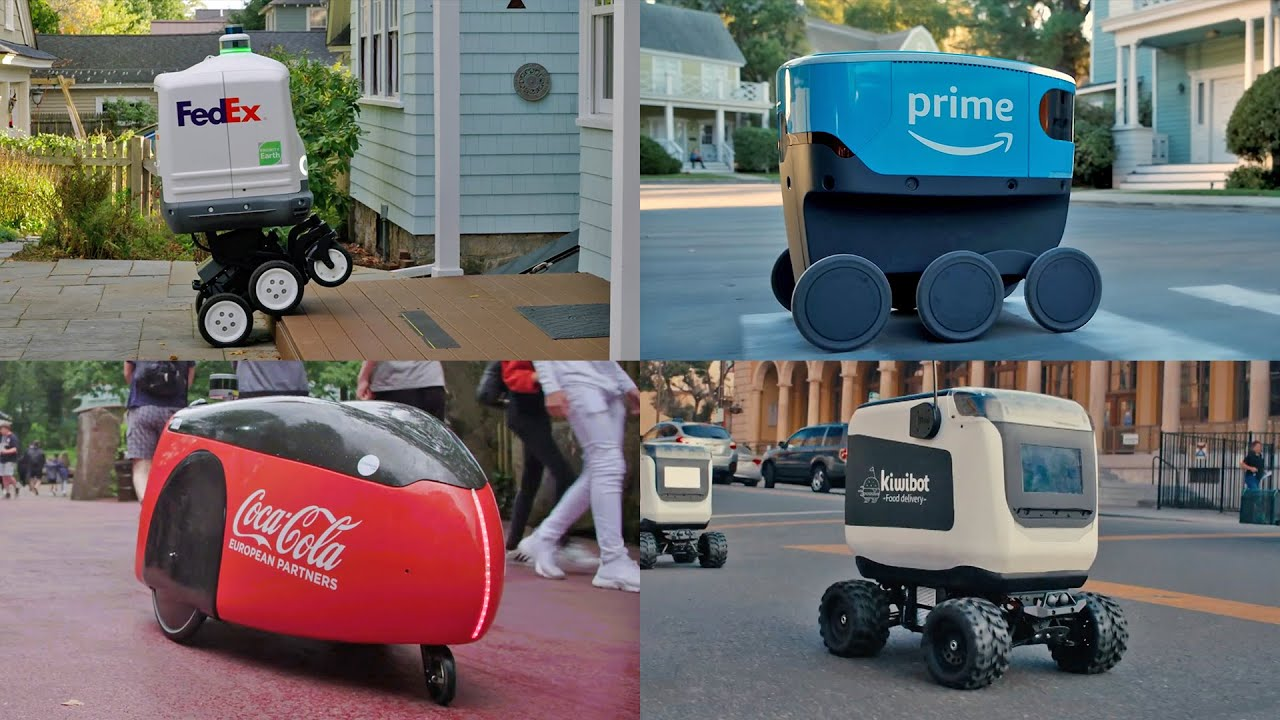
\includegraphics[width=0.37\linewidth]{Figures/delivery_robots.jpg}}
            \hspace{0.3pt}
            \subfloat[Transporting products~\cite{WarehouseRobots, coltin2013online}]{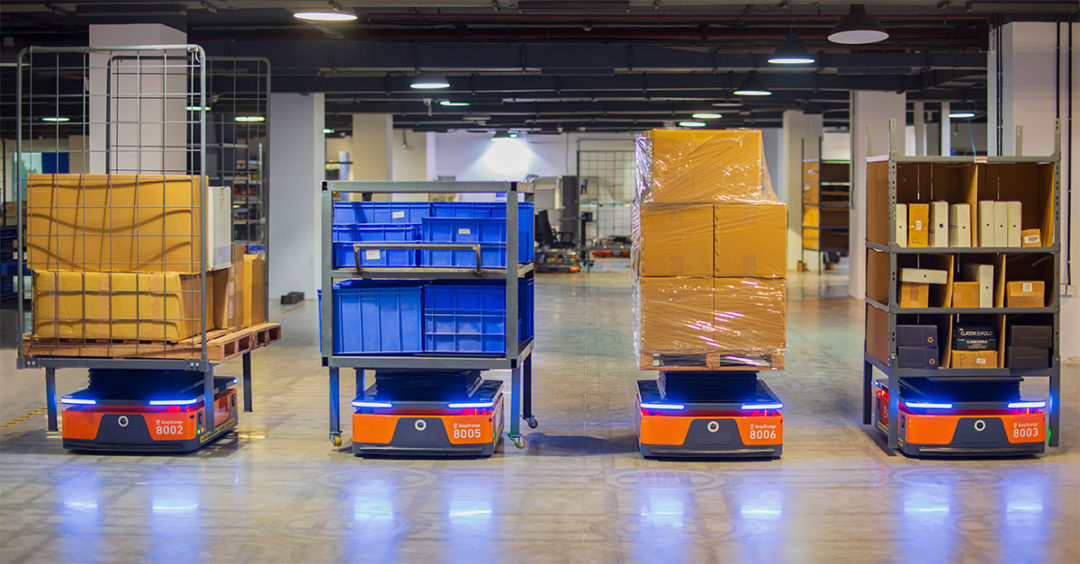
\includegraphics[width=0.4\linewidth]{Figures/warehouse robots.jpg}}
            \vfill
            \subfloat[Wildfire tracking and management~\cite{DronesWildfire,chen2024drone}]{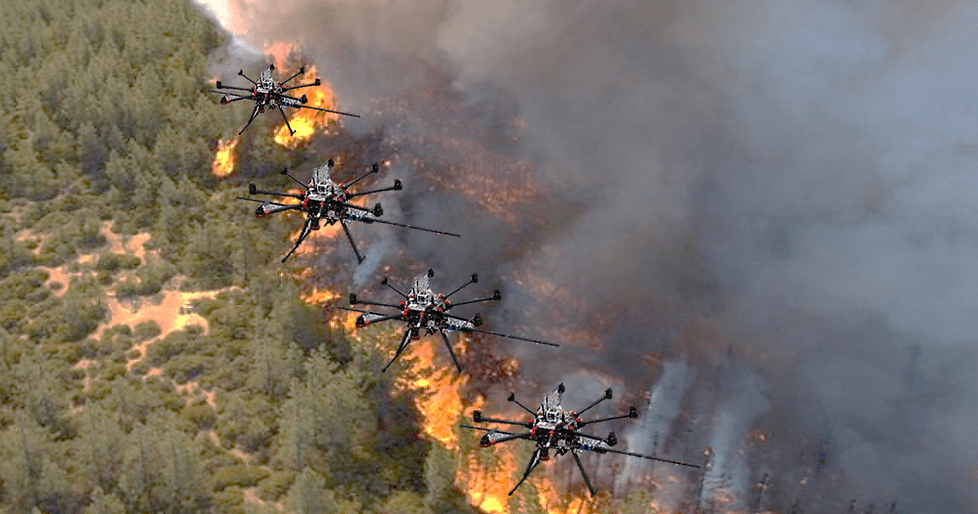
\includegraphics[width=0.37\linewidth]{Figures/Drones-and-wildfire.png}}
            \hspace{0.3pt}
            % \subfloat[Search and rescue operations ~\cite{SearchRescue}]{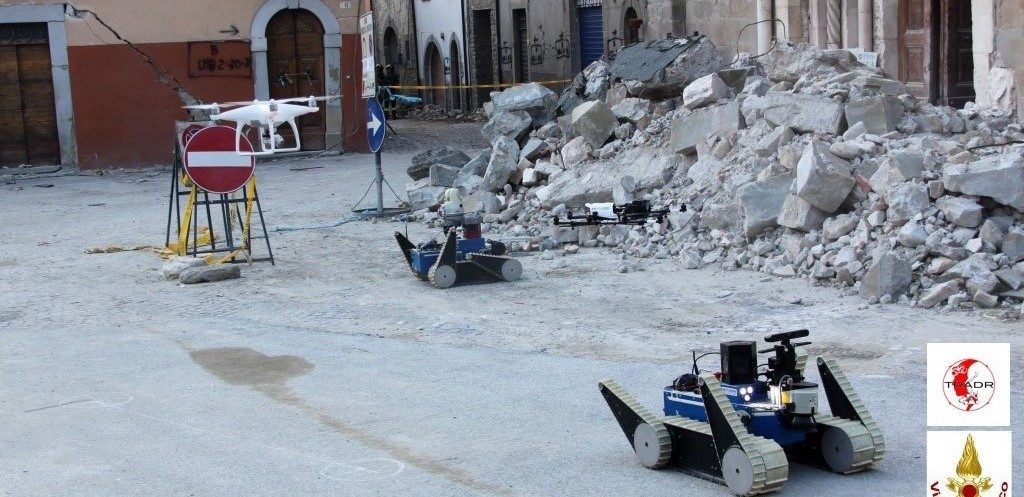
\includegraphics[width=0.4\linewidth]{Figures/search_rescue.jpg}}
        \end{figure}
        % \begin{figure}
        %     \centering
        %     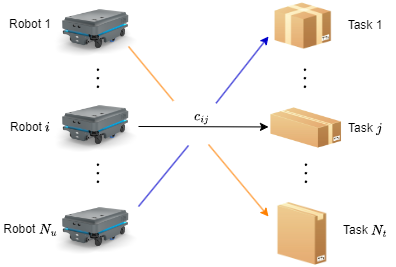
\includegraphics[width=0.5\linewidth]{Figures/Single assignment problem.png}
        % \end{figure}
    \end{itemize}
\end{frame}

%%%%%%%%%%%%%%%%%%% Background
%%%%%%%%%%%%%%%%%%%

\begin{frame}{Literature Review - Formulation}
\begin{itemize}
    \item Combinatorial optimization problem with binary decision variables $x_{ij}$
\end{itemize}
 \vspace{4pt}
    \begin{columns}
    \begin{column}{0.65\textwidth}
    % \begin{itemize}
        % \item Combinatorial optimization problem with binary decision variables $x_{ij}$, \\
        \begin{subequations}
            \label{eq_opt_problem}
            \begin{align}
            \redpause
            & \max \quad \sum_{i=1}^{N_u} \sum_{j=1}^{N_t} \tikzmarknode[uwpurple]{cij}{c_{ij}}(\mathbf{x}_i, \tikzmarknode[uwpurple]{p_i}{\mathbf{p}_i})\cdot x_{ij} \\ \redpause
            & \text{s.t} \quad \sum_{j=1}^{N_t} x_{ij} \leq \tikzmarknode[uwpurple]{L_t}{L_t} \quad \forall i \in %\mathcal{I} \triangleq 
            \{1,\cdots,N_u\}, \\ \redpause
            & \qquad \sum_{i=1}^{N_u} x_{ij} \leq 1 \quad \forall j \in %\mathcal{J} \triangleq 
            \{1,\cdots,N_t\}, \\ \redpause
            & \qquad \sum_{i=1}^{N_u} \sum_{j=1}^{N_t} x_{ij} = 
            %N_{\min} \triangleq 
            \min \{N_t, N_u\cdot L_t\}  \\ \redpause
            & \qquad x_{ij} \in \{0, 1\} \quad \forall (i,j) 
            %  \in \mathcal{I} \times \mathcal{J},
            \end{align}
        \end{subequations}
        \begin{tikzpicture}[overlay, remember picture]
            \onslide<1->
            \node[above right=0.36cm and -2.5cm of cij, align=center, color=uwpurple] (label) {\footnotesize score function: reward for robot $i$ completing task $j$};
            \draw[->, thick, uwpurple] (label) -- (cij);
            \node[below right=0.36cm and -1.8cm of p_i, align=center, color=uwpurple] (label2) {\footnotesize path vector (order of task execution) };
            \draw[->, thick, uwpurple] (label2) -- (p_i);
            \onslide<2->
            \node[below right=0.36cm and -1.0cm of L_t, align=center, color=uwpurple] (label3) {\footnotesize max. \# of tasks each robot can get};
            \draw[->, thick, uwpurple] (label3) -- (L_t);
        \end{tikzpicture}
        \onslide<5->
        % \item Can be more general (e.g., robot coalitions)
    % \end{itemize}
    \end{column}
    \begin{column}{0.55\textwidth}
        % \begin{figure}
        %     {
        %     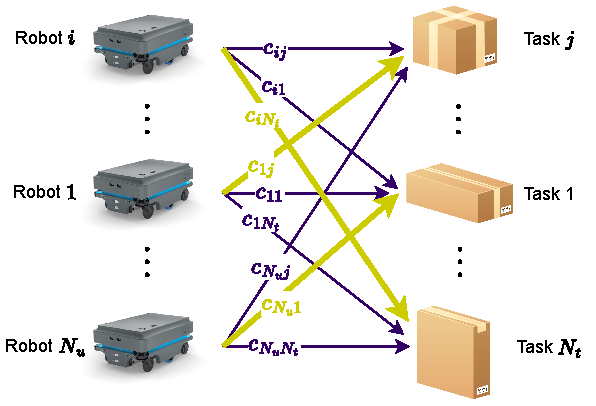
\includegraphics[width=0.62\linewidth]{Figures/LinearAssign.pdf}}
        %     \caption{Linear single assignment ($L_t=1$) with constant score values}
        % \end{figure}
        \begin{figure}
            \centering
            \onslide<1->
            \subfloat[Linear single assignment ($L_t=1$) with constant score values ]{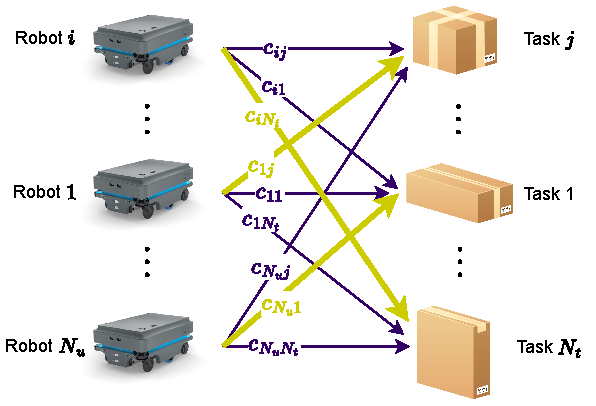
\includegraphics[width=0.85\linewidth]{Figures/LinearAssign.pdf}}
            \addtocounter{subfigure}{-1}
            \vfill
        % \label{fig:1}
        \end{figure}
    \end{column}
    \end{columns}
\end{frame}

%%%%%%%%%%%%%%%%%%% Applications
%%%%%%%%%%%%%%%%%%%
\begin{frame}{Literature Review - Centralized MRTA}
    \begin{columns}
    \begin{column}{0.65\textwidth}
    \begin{itemize}
        % \item Centralized task assignment (TA)
        \item Task assignment (TA) is NP-Hard~\cite{karp2010reducibility} (even the linear TA)
        \item Linear assignment $c_{ij}(\mathbf{x}_i,{\mathbf{p}_i}) = c_{ij}$ 
        \begin{itemize}
            \item Can be solved efficiently in some cases~\cite{bertsekas1991linear}
            \item Linear program relaxation: $x_{ij} \in \{0, 1\}$ to $0\le x_{ij} \le 1$
            \item Hungarian method~\cite{kuhn1955hungarian}, auction algorithm~\cite{bertsekas1988auction}
        \end{itemize}
        \vspace{0.4cm}
        \pause
        \item Nonlinear assignment
        \begin{itemize}
            \item Exact methods: dynamic programming~\cite{pardalos1999nonlinear}, branch and bound ~\cite{dyer1986linear} (exponential complexity)
            \item Approximate methods: convex relaxations~\cite{ma2015efficient}, greedy algorithms~\cite{romeijn2000class}
            % \item For example, $c_{ij}(\mathbf{x}_i,{\mathbf{p}_i})$ can be the probability that a set of robots successfully complete a task~\cite{haight2000integer} 
        \end{itemize}
    \end{itemize}
    \end{column}
    \begin{column}{0.5\textwidth}
    \begin{figure}
        \centering
        \onslide<1->
        \subfloat[Linear MRTA (one to one)]{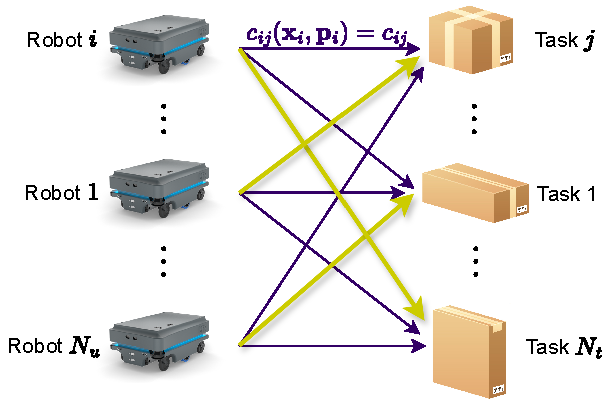
\includegraphics[width=0.8\linewidth]{Figures/LinearAssign_2.pdf}}
        \vfill
        \visible<2>{
        \subfloat[Nonlinear MRTA (robot coalitions)]{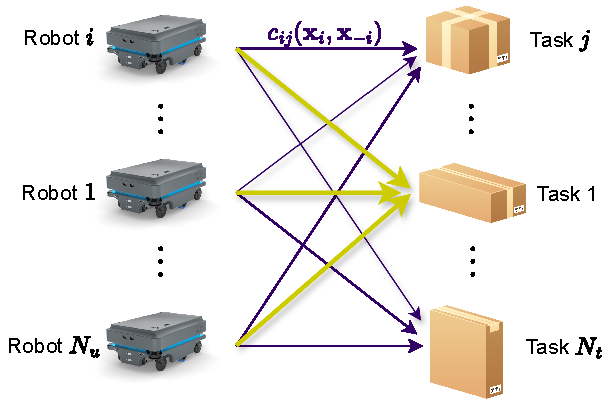
\includegraphics[width=0.8\linewidth]{Figures/nonlinearAssign.pdf}}
        }
    % \label{fig:1}
    \addtocounter{subfigure}{-1}
    \end{figure}
    \end{column}
    \end{columns}
\end{frame}

\begin{frame}{Literature Review - Decentralized MRTA}
    \begin{itemize}
        \item Decentralized MRTA methods are becoming more relevant
        \begin{itemize}
            \item Computationally efficient~\cite{choi2009consensus}; robust~\cite{chopra2017distributed}; scalable~\cite{shorinwa2023distributed}
        \end{itemize}
        % \item Derived from their centralized counterpart
        % \item Implicit methods: coordination on local information
        % \item Explicit methods: coordination on local understanding of assignments
    \end{itemize}

    \begin{block}{~\vspace{0.2cm}}
        \begin{center}
        \vspace{-1.0cm}
        \setcellgapes{3pt}\makegapedcells
        \begin{tabular}{>{\centering}p{0.45\textwidth}|>{\centering\arraybackslash}p{0.45\textwidth}}
         \textcolor{white}{\bfseries\boldmath Implicit methods~\cite{alighanbari2005decentralized, curtis2003simultaneous, samiei2023distributed}} & \textcolor{white}{\bfseries Explicit methods~\cite{arslan2007autonomous,choi2009consensus,johnson2017decentralized, shorinwa2023distributed, qu2019distributed}} \\
        consensus on information 
        (e.g., task positions) 
        % to compute score function matrix $C(\mathbf{p},\mathbf{x})\in \reals^{N_u \times N_t}$ 
        & consensus on local understanding of assignments \\ 
        solve local copy of the entire MRTA to get $\mathbf{x}\in \{0,1\}^{N_u \times N_t}$&  each robot solves only for its local assignments $\mathbf{x}_i \in \{0,1\}^{N_t}$
        % either solve a local copy of the entire MRTA to get $\mathbf{x}$ or each robot's local assignments $\mathbf{x}_i \in \{0,1\}^{N_t}$
        \\ \hline
        \begin{itemize}
            \item {\color{ao} high global reward}
            \item {\color{red}conflicting assignments if inaccurate information}
            \item {\color{red}computationally inefficient} 
        \end{itemize}
        &
        \begin{itemize}
            \item {\color{ao}computationally efficient}
            \item {\color{ao}conflict-free assignments}
            \item {\color{red} low global reward because assignments are based on local information}
        \end{itemize}
        
        \end{tabular}
        \end{center}
    \end{block}
\end{frame}

% \begin{frame}{Literature Review - Implicit methods}
%     \begin{columns}
%     \begin{column}{0.6\textwidth}
%     \begin{itemize}
%         \item Distributed Hungarian algorithm~\cite{samiei2023distributed} (similarly~\cite{alighanbari2005decentralized})
%         \begin{itemize}
%             \item Step 1: communicate local information to converge on global information
%             \item Step 2: build score/cost matrix and solve the Hungarian algorithm 
%         \end{itemize}
%         \item {\color{green}Achieves assignments with high global reward}
%         \item {\color{red}Conflicting assignments if inaccurate information communication}
%         \item {\color{red}Computationally inefficient}
%     \end{itemize}
%     \end{column}
%     \begin{column}{0.55\textwidth}
%     \begin{figure}
%         \centering
%         \onslide<1->
%         \subfloat[Communication]{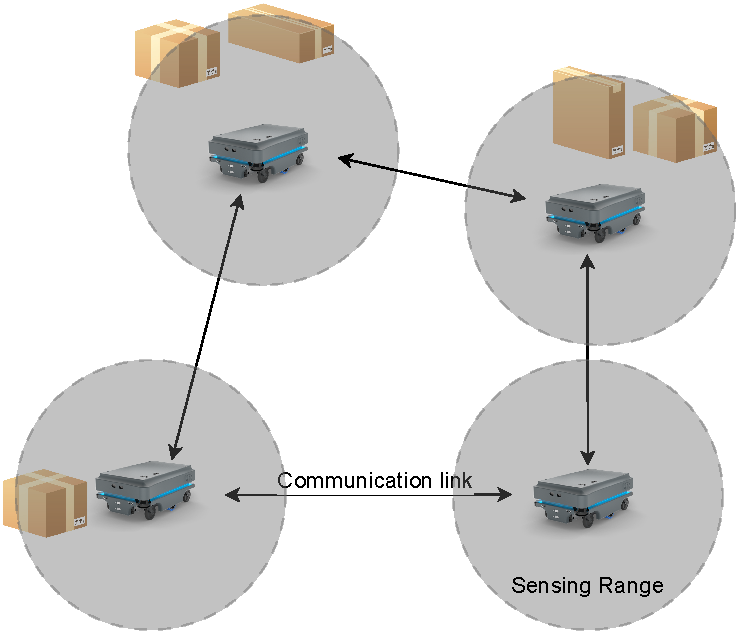
\includegraphics[width=0.7\linewidth]{Figures/communication.pdf}}
%         \vfill
%         \subfloat[Solve locally]{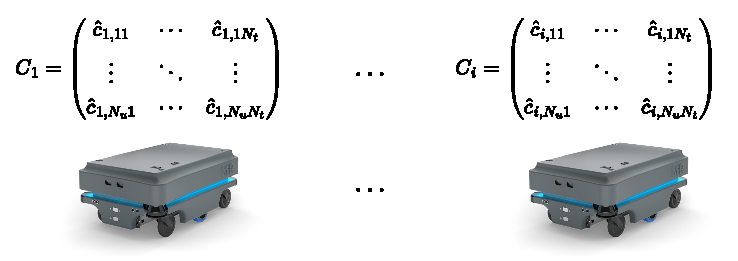
\includegraphics[width=1.\linewidth]{Figures/score_matrices.pdf}}
%     \label{fig:2}
%     \end{figure}
%     \end{column}
%     \end{columns}
% \end{frame}

% \begin{frame}{Literature Review - Explicit methods}
%     \begin{columns}
%     \begin{column}{0.6\textwidth}
%     \begin{itemize}
%         \item Distributed auction algorithms~\cite{choi2009consensus},Game-theoretic~\cite{arslan2007autonomous}, and distributed optimization methods~\cite{shorinwa2023distributed, camisa2022multi}
%         \item High-level idea:
%         \begin{itemize}
%             \item Step 1: each robot locally chooses an assignment 
%             \item Step 2: communicate assignments to resolve conflicts 
%         \end{itemize}
%         \item {\color{green}Computationally efficient}
%         \item {\color{green}Conflict-free assignments}
%         \item {\color{red}Base their assignments on their local information or assume information is globally known}
%     \end{itemize}
%     \end{column}
%     \begin{column}{0.55\textwidth}
%     \begin{figure}
%         \centering
%         \onslide<1->
%         \subfloat[Communication]{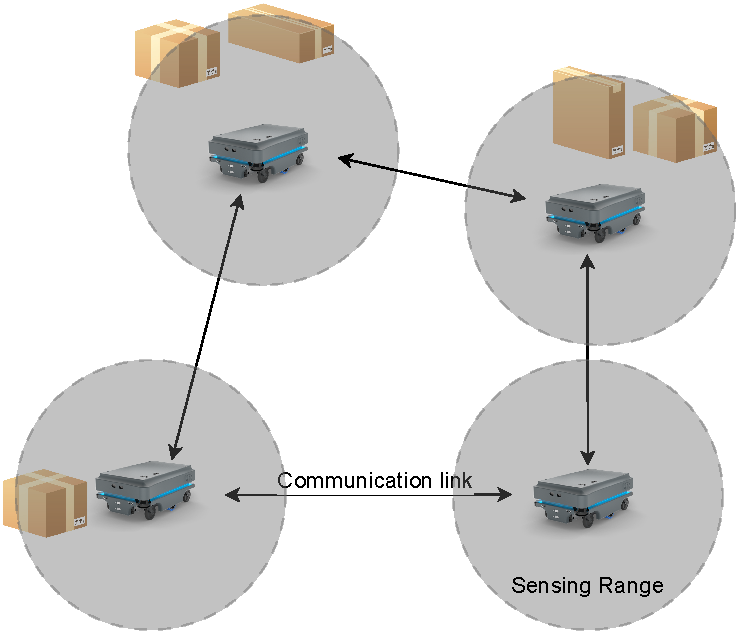
\includegraphics[width=0.7\linewidth]{Figures/communication.pdf}}
%         \vfill
%     \label{fig:2}
%     \end{figure}
%     \end{column}
%     \end{columns}
% \end{frame}